\documentclass[11pt]{report}
\usepackage{graphicx}
\usepackage{tabularx}
\usepackage{graphicx}
\usepackage[margin=0.5in]{geometry}
\usepackage{listings,xcolor}
\usepackage{tcolorbox}
\usepackage{multicol}
\tcbuselibrary{listings,skins}
\lstset{
    string=[s]{"}{"},
    stringstyle=\color{blue},
    comment=[l]{:},
    commentstyle=\color{black},
    breaklines=true,
}
\lstdefinestyle{mystyle}{
numbers=left, 
numberstyle=\small, 
numbersep=4pt, 
language=Python
}
\newtcblisting{mylisting}[2][]{
    arc=0pt, outer arc=0pt,
    listing only, 
    listing style=mystyle,
    title=#2,
    #1
    }
\PassOptionsToPackage{hyphens}{url}\usepackage{hyperref}
\begin{document}

\title{Assignment 7}
\author{Joshua Graham}

\maketitle
\pagebreak
\begin{abstract}
All Scripts used in the assignment can be found in the A7 folder, if needed.

\end{abstract}
\section{Problem 1}
	Question 1 was mainly to download the blogs and run the given code on them to generate the blogdata1.txt file. I decided it would be easy to do with a one-liner in bash so I wrote up a command to do it. Halfway in to the second question I realized I had several duplicates, so I came back and rewrote the command to generate a list of unique blogs. I added the two required urls at this point. 
\begin{mylisting}[hbox,enhanced,drop shadow]{Generating links}
touch blogs.txt; while ["$(wc -l blogs.txt)" -lt 199 ]; do echo "Iteration: $i"; echo "$(curl -L -s -o /dev/null -w %{url_effective} 'http://www.blogger.com/next-blog?navBar=true&blogID=3471633091411211117')" | sed -n -e "s/?expref=next-blog//p" | tee -a blogs.txt; cat blogs.txt | sort | uniq > hold; mv hold blogs.txt; done
\end{mylisting}

This dealt with a lot of the work, but I still needed to append the text required for the feed parser. I did that with:

\begin{mylisting}[hbox,enhanced,drop shadow]{Formatting links}
while read line; do echo $line\feeds/posts/default; done < blogs.txt > feeds.txt
\end{mylisting}



The second part of this question was to run the given code to generate blogdata1.txt. There wasn't anything specifically special to mention about this step, it just took using the code correctly, which can be shown below. 

\begin{mylisting}[hbox,enhanced,drop shadow]{Generating blogdata1.txt}
apcount = {}
wordcounts = {}
feedlist = [line for line in open('blogs.txt', 'r')]
for feedurl in feedlist:
    try:
        (title, wc) = getwordcounts(feedurl)
        wordcounts[title] = wc
        for (word, count) in wc.items():
            apcount.setdefault(word, 0)
            if count > 1:
                apcount[word] += 1
    except:
        print('Failed to parse feed %s' % feedurl)

wordlist = []
for (w, bc) in apcount.items():
    frac = float(bc) / len(feedlist)
    if frac > 0.1 and frac < 0.5:
        wordlist.append(w)

out = open('blogdata1.txt', 'w')
out.write('Blog')
for word in wordlist:
    out.write('\t%s' % word)
out.write('\n')
for (blog, wc) in wordcounts.items():
    print(blog)
    out.write(blog)
    for word in wordlist:
        if word in wc: 
            out.write('\t%d' % wc[word])
        else:
            out.write('\t0')
    out.write('\n')

\end{mylisting}
 This code did not work on every link. The below listed links, for whatever reason, failed to parse. Because of this they were not listed in the set of data.
\begin{mylisting}[hbox,enhanced,drop shadow]{Failed Links}
Failed to parse feed http://globalgoon.blogspot.com/feeds/posts/default
Failed to parse feed http://www.chrisanne-grise.com/feeds/posts/default
Failed to parse feed http://www.confessionsofamusicaddict.com/feeds/posts/default
Failed to parse feed http://www.holaolamusic.com/feeds/posts/default
Failed to parse feed http://www.punkrockteaching.org/feeds/posts/default
Failed to parse feed http://www.samtasticreview.com/feeds/posts/default
Failed to parse feed http://www.sunstockmusic.com/feeds/posts/default
\end{mylisting}
Here are the first 10 titles of the blogs. The rest can be found in the blognames.txt file.

\pagebreak
\begin{itemize}
\item 300 Vinyl Challenge 2017
\item Indie, Rock And Other Great Music
\item She's mad but she's magic. There's no lie in her fire.
\item Abu Everyday
\item adrianoblog
\item A H T A P O T
\item A layer of chips
\item ALL MY BROTHERS AND SISTERS
\item A Music History by Wayne R. Flower
\item Andrea Jesse's Favorite Songs
\end{itemize}
\pagebreak
\section{Problem 2}
Question 2 was basically correctly executing the code. This was the easiest of the three questions. The file dendrogram.py generates the jpeg file as well as prints the ascii dendrogram to stdout. The last two lines in the output of dendrogram.py are the failed blogs. In my example, two blogs failed. They are not included in the dendrograms. \textbf{The ascii text is too difficult to format correctly into this document. It can be found in the file ascii.txt. The image for the jpeg can be found in clusters.jpg. It is scaled to about 15\% its usual size to allow it to fit on the page.}


\fbox{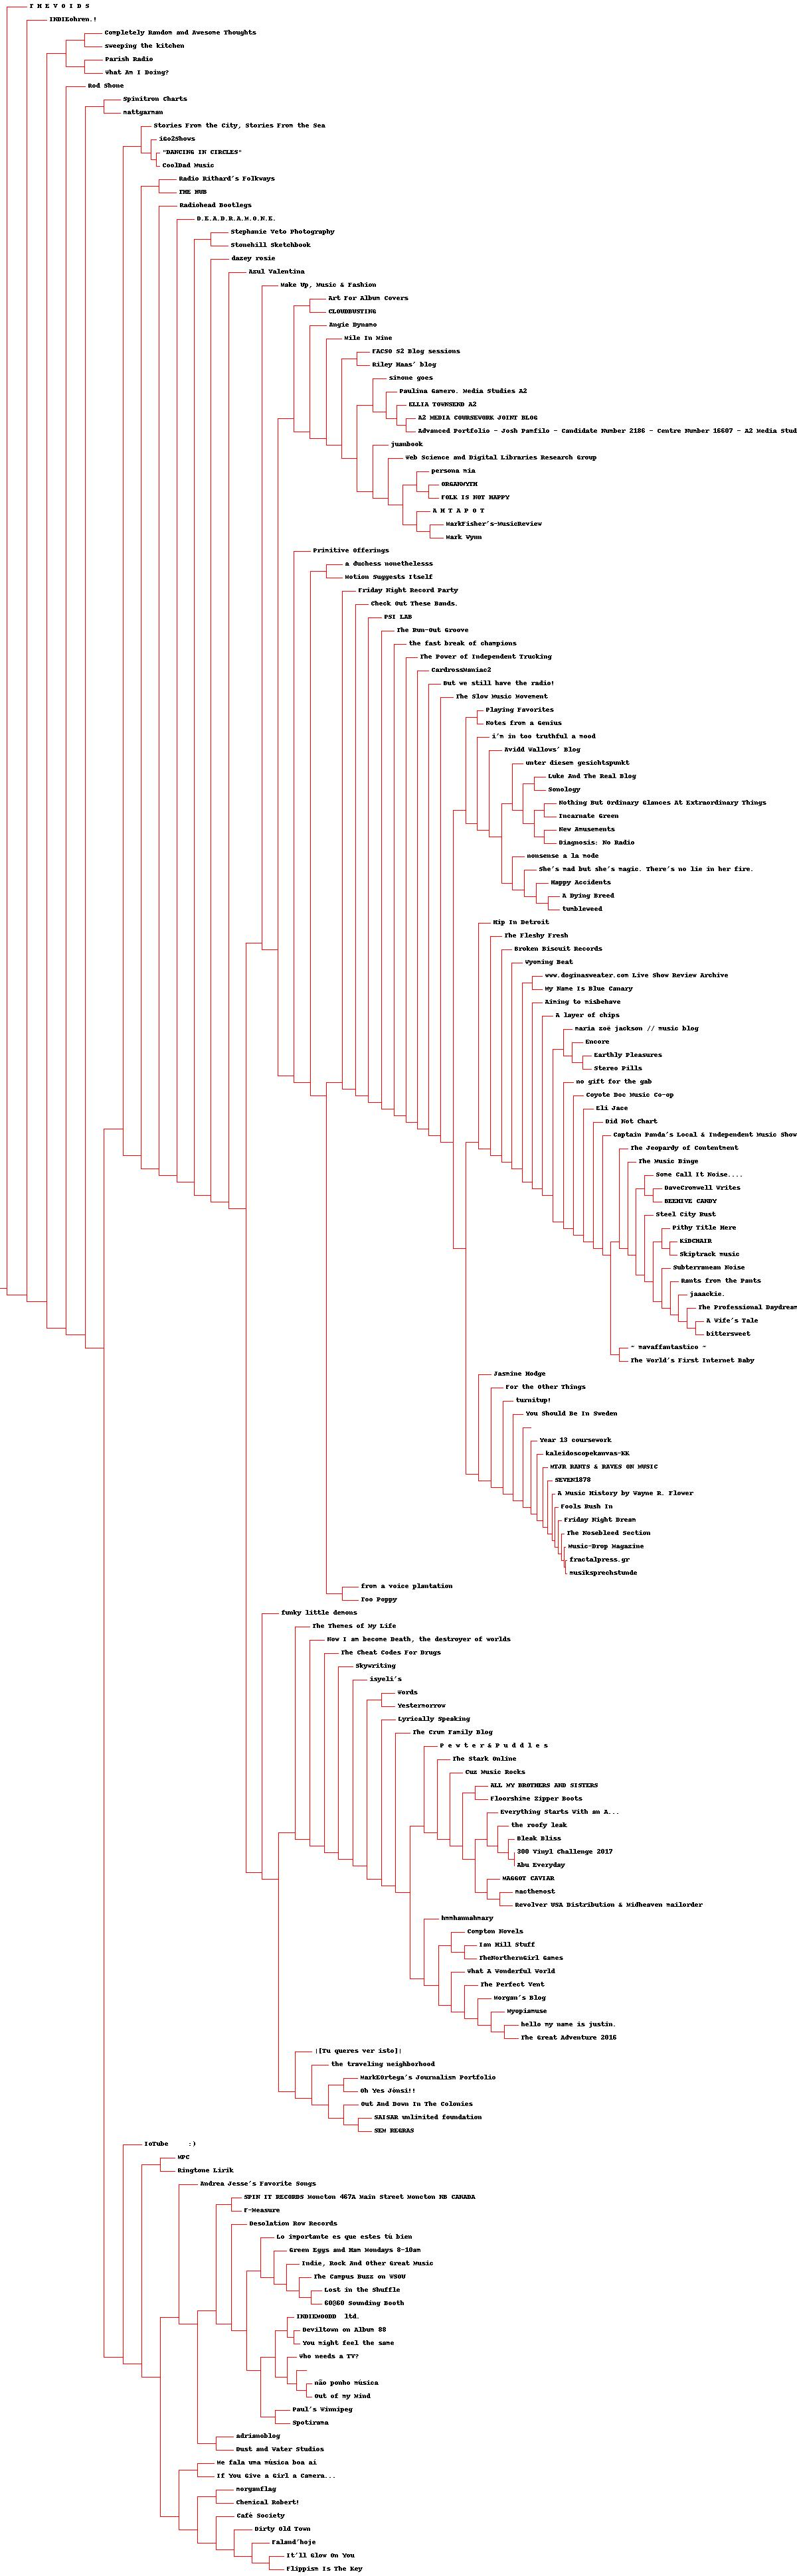
\includegraphics[scale=0.15]{clusters.jpg}}

\pagebreak
\section{Problem 3}
Question 3 was to use k-means to generate centroids for the data. Again, this was just using the code given to use, but minor conversions had to be done from python2 syntax to python3 syntax. The amount of iterations are shown in the list below. And the centroids printed out for each set are found in their respective tables. \textbf{Code for this question can be found in kmeans.py}

\begin{itemize}
\item When k=5 it took 7 iterations. 
\item When k=10 it took 9 iterations.
\item When k=20 it took 8 iterations. 
\end{itemize}
\begin{mylisting}[hbox,enhanced,drop shadow]{K at 5}
[1, 3, 4, 5, 17, 35, 38, 42, 46, 48, 62, 80, 93, 94, 97, 99, 107, 108, 117, 127, 131, 135, 136, 141, 147, 148, 159]
[2, 10, 12, 13, 14, 18, 22, 24, 26, 28, 31, 33, 39, 47, 56, 57, 58, 59, 60, 63, 64, 65, 66, 69, 72, 73, 75, 76, 77, 78, 79, 81, 85, 86, 90, 91, 96, 100, 102, 105, 106, 109, 111, 112, 113, 114, 118, 122, 123, 129, 133, 138, 139, 144, 149, 152, 153, 156, 157, 160, 161, 164, 167, 169, 172, 173, 178, 179, 181, 183, 187]
[8, 51, 52, 53, 54, 71, 74, 98, 101, 103, 104, 125, 137, 150, 170, 174, 190]
[0, 6, 7, 11, 15, 19, 21, 23, 25, 27, 29, 30, 36, 37, 40, 41, 43, 44, 45, 49, 50, 55, 61, 67, 68, 70, 82, 83, 84, 87, 88, 89, 92, 95, 110, 115, 116, 119, 120, 121, 124, 126, 128, 130, 132, 140, 142, 143, 145, 146, 151, 154, 155, 158, 162, 163, 165, 166, 168, 171, 175, 176, 177, 184, 185, 186, 188, 189, 191, 193]
[9, 16, 20, 32, 34, 134, 180, 182, 192]
\end{mylisting}
\begin{mylisting}[hbox,enhanced,drop shadow]{K at 10}
[3, 5, 35, 38, 42, 48, 62, 93, 94, 99, 107, 108, 131, 136, 147, 159]
[8, 51, 52, 53, 54, 71, 74, 101, 103, 104, 137, 170, 174, 190]
[1, 4, 9, 17, 20, 32, 80, 97, 98, 117, 127, 134, 135, 141, 142, 148, 150, 163, 180, 182]
[16, 34, 192]
[0, 6, 7, 15, 19, 21, 23, 25, 27, 30, 36, 37, 40, 41, 43, 45, 49, 50, 66, 67, 76, 82, 83, 84, 87, 88, 89, 110, 115, 121, 124, 128, 130, 132, 143, 145, 146, 151, 155, 158, 162, 165, 166, 167, 171, 175, 184, 185, 186, 188, 189, 191]
[29, 69, 154, 176]
[61, 125]
[11, 60, 65, 100, 116, 119, 126, 152, 168, 187, 193]
[2, 10, 12, 13, 14, 18, 22, 24, 26, 28, 31, 33, 39, 47, 56, 57, 58, 59, 63, 64, 72, 73, 75, 77, 78, 79, 81, 86, 90, 91, 95, 96, 102, 105, 106, 109, 111, 112, 113, 114, 118, 122, 123, 129, 133, 138, 139, 144, 149, 153, 156, 157, 160, 161, 164, 169, 172, 173, 177, 178, 179, 181, 183]
[44, 46, 55, 68, 70, 85, 92, 120, 140]
\end{mylisting}
\begin{mylisting}[hbox,enhanced,drop shadow]{K at 20}
[3, 170, 174]
[11, 35, 55, 62, 89, 147, 148, 159, 193]
[67, 112]
[38, 44, 47, 68, 70, 92, 93, 105, 107, 108, 120, 140, 182]
[5, 31, 32, 46, 69, 88, 116, 117, 126, 127, 131, 135, 136, 153, 172]
[71, 101, 103, 137]
[2, 10, 12, 13, 14, 24, 28, 33, 56, 58, 63, 64, 73, 75, 77, 78, 79, 81, 86, 90, 91, 96, 111, 114, 118, 129, 133, 138, 144, 149, 157, 160, 183]
[18, 22, 26, 72, 76, 85, 95, 106, 109, 122, 123, 151, 156, 161, 167, 169, 173, 181, 185]
[6, 37, 39, 57, 66, 113, 119, 128, 132, 146, 162, 164, 166, 177, 189]
[102]
[19, 110, 115, 130, 155, 191, 192]
[0, 7, 15, 21, 23, 25, 27, 30, 36, 40, 41, 43, 45, 49, 50, 82, 83, 84, 87, 99, 121, 124, 143, 145, 158, 165, 168, 171, 175, 184, 186, 188]
[29, 61, 154, 176]
[42, 59, 65, 94, 139, 152, 178, 179, 180, 187]
[125]
[8, 51, 52, 53, 54, 74, 104, 190]
[48, 60, 100]
[1, 4, 9, 17, 20, 80, 97, 98, 134, 141, 142, 150, 163]
[]
[16, 34]
\end{mylisting}
\pagebreak
\section{Problem 4}
I could not do question 4. I had an error that involved dividing by zero, and for the life of me I could not figure it out. Here is the code I added to the original clusters.py file, now renamed mds.py.

\begin{mylisting}[hbox,enhanced,drop shadow]{MDS code.}
 rows, cols, data = readfile("blogdata1.txt")
 coords=scaledown(data)
 draw2d(coords,rows, jpeg='blogs2d.jpg')

\end{mylisting}
\end{document}